\documentclass[12pt, oneside]{article} 
\usepackage{amsmath, amsthm, amssymb, calrsfs, wasysym, verbatim, bbm, color, graphics, geometry, multirow, booktabs}
\usepackage{graphicx}
\usepackage{tikz}
\usepackage{amsmath}
\usepackage{graphicx}
\usepackage{amsmath, amssymb, amsthm}
\usepackage{setspace}
\usepackage{tikz}
\usetikzlibrary{trees, positioning}
\usepackage{pgfplots}
\renewcommand{\baselinestretch}{1.0}
\geometry{tmargin=.75in, bmargin=.75in, lmargin=.75in, rmargin = .75in}  

\newcommand{\R}{\mathbb{R}}
\newcommand{\C}{\mathbb{C}}
\newcommand{\Z}{\mathbb{Z}}
\newcommand{\N}{\mathbb{N}}
\newcommand{\Q}{\mathbb{Q}}
\newcommand{\Cdot}{\boldsymbol{\cdot}}


\title{SP25 8732: Homework 3}
\author{Danbo CHEN}
\date{\today}

\begin{document}

\maketitle
\vspace{.25in}

\section{Question 1}
\textbf{(a) Solution:}

\begin{center}
    
    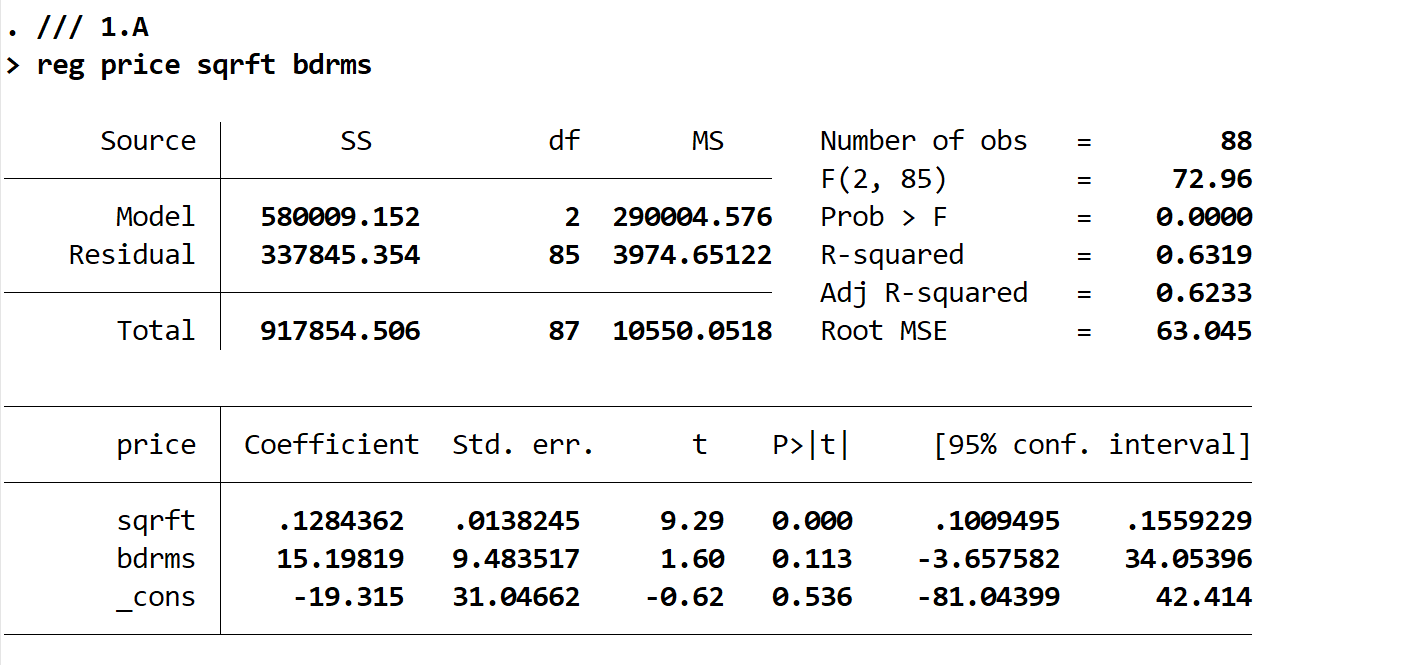
\includegraphics[width=0.8\textwidth]{Figure/P1.A.jpg}

    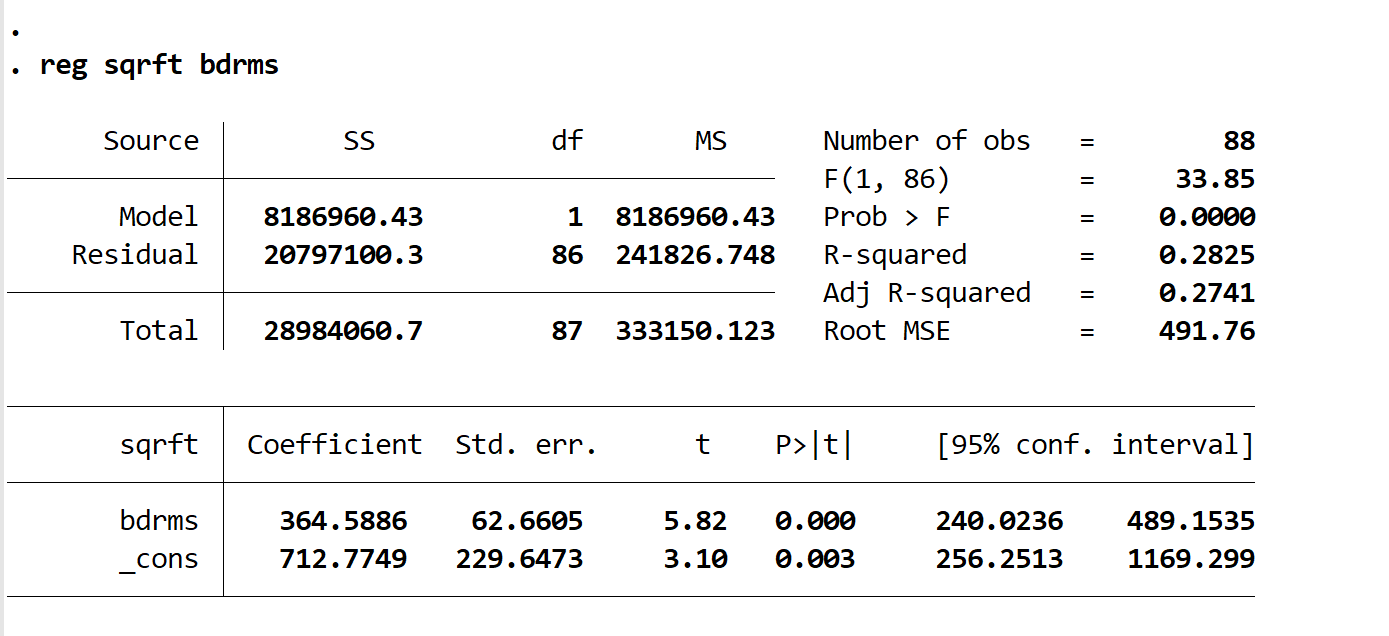
\includegraphics[width=0.8\textwidth]{Figure/P1.B.jpg}

    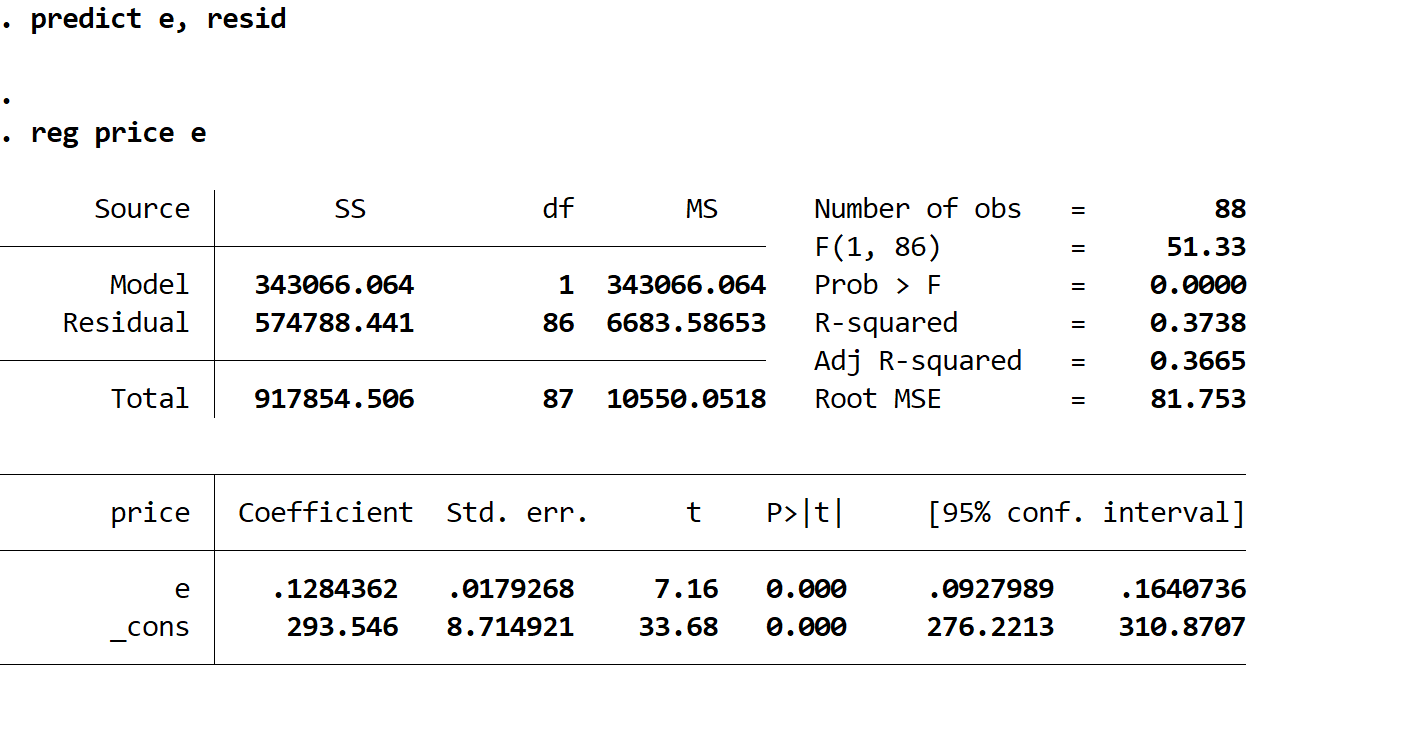
\includegraphics[width=0.8\textwidth]{Figure/P1.C.jpg}

\end{center}


\section{Question 2}
\textbf{Solution:}

For a general model \( Y = X\beta + \epsilon \) with instruments \( Z \), the reduced form equations are:

\[
Y = Z\lambda + v,
\]

\[
X = Z\Gamma + U.
\]

For identification, we need \( \text{rank}(\Gamma) = K \) where \( K = 3 \).

Let's focus on the demand equation first. We have \( X = [1, P, Y] \) and \( Z = [1, Y, W] \). The reduced form for \( X \) is:

\[
X = Z\Gamma + U
\]

or

\[
\begin{bmatrix} 1 & P & Y \end{bmatrix} = \begin{bmatrix} 1 & Y & W \end{bmatrix}
\begin{bmatrix} 
1 & \gamma_1 & 0 \\ 
0 & \gamma_2 & 1 \\ 
0 & \gamma_3 & 0 
\end{bmatrix} + U.
\]

Expanding the equation for \( P \):

\[
P = \gamma_1 + \gamma_2 Y + \gamma_3 W.
\]

Hence, \( \Gamma \) has full rank (and \( \alpha \) is identified) as long as \( \gamma_3 \neq 0 \).

Similarly, for the supply equation, we have \( X = [1, P, W] \) and \( Z = [1, W, Y] \). The reduced form for \( X \) is:

\[
\begin{bmatrix} 1 & P & W \end{bmatrix} = \begin{bmatrix} 1 & W & Y \end{bmatrix}
\begin{bmatrix} 
1 & \gamma_1 & 0 \\ 
0 & \gamma_2 & 1 \\ 
0 & \gamma_3 & 0 
\end{bmatrix} + U.
\]

Thus, \( \beta \) is identified (i.e., \( \Gamma \) has full rank) if \( \gamma_3 \neq 0 \).


\end{document}